\documentclass[a4paper,11pt]{article}

\usepackage[T1]{fontenc}
\usepackage[utf8]{inputenc}
\usepackage[francais]{babel}
\usepackage{lmodern}
\usepackage{amsmath}
\usepackage{graphicx}
\setlength\abovecaptionskip{0.10ex}
\usepackage{titling}
\setlength{\droptitle}{-4cm}
\usepackage{fullpage}
\RequirePackage{graphicx}
\DeclareGraphicsExtensions{.pdf,.jpg,.png,.JPG}
\RequirePackage{float}

\newcommand{\InsertFig}[1]{
\begin{figure}[H]
\begin{center}
\includegraphics[width=.75\textwidth]{img/#1}
\end{center}
\end{figure}}
\newcommand{\InsertFigTitle}[2]{
\begin{figure}[H]
\caption{#2}
\begin{center}
\includegraphics[width=.75\textwidth]{img/#1}
\end{center}
\end{figure}}

\title{Rapport SY19 TP01 - Positionnement Multidimensionnel}
\author{Thomas ABASSI \& Joan MOESCH}

\begin{document}
\maketitle

\section{Exercice Theorique}
\noindent Le but de ce TP est d'entreprendre l'analyse dimmensionnelle de donnees a travers differents outils tel que l'ACP ou l'AFTD. Apres application de ces outils sur un exercice theorique, nous utliserons ces differentes techniques sur des donnees d'applications. \\

\noindent D'autre part, nous utiliserons plusieurs moyens de projections tels que celles de Sammon et Kruskal ou encore les diagrammes de Shepard afin de comparer les resultats des outils ennonces precedemment.
\section{Exercice Theorique}

\subsection{ACP}

\subsubsection{Axes factoriels et pourcentages d'inertie expliquee}

\noindent Apres s'etre assure que la matrice X est bien centree en colonne, on procede a l'analyse spectrale de la matrice $S = \frac{1}{8} X^T X $. Les vecteurs propres nous donnent les axes factoriels : 
\begin{center}
$U = \begin{pmatrix}
-0.8472171&-0.5312469\\
0.5312469&-0.8472171\\
\end{pmatrix}$
\end{center}


\noindent En mesurant l'importance de chaque valeur propre de S, on obtient le pourcentage d'inertie expliquee par chacun des axes :
\begin{center}
- Axe 1 : $E1 = \frac{\lambda_1}{\lambda_1 + \lambda_2} * 100 = 98.44709 \%$\\
- Axe 2 : $E2 = \frac{\lambda_2}{\lambda_1 + \lambda_2} * 100 = 1.552913 \%$\\
\end{center}
\noindent C'est donc le premier axe qui explique la quasi totalite des donnees.\\

\subsubsection{Composantes principales et représentation dans le premier plan factoriel}

\noindent Si on projet notre nuage initial X sur les axes factoriels (vecteurs propres de S), nous obtenons la matrice des composantes principales $C = XU$ :
\begin{center}
$ C =  \begin{pmatrix}
-6.4044746&-5.786424\\
-0.3090252&-6.095449\\
1.7586707&-6.569405\\
-7.2516917&-6.317671\\
-5.8732278&-6.633641\\
0.9114536&-7.100652\\
-6.2968363&-6.899265\\
1.2274238&-5.722188\\
\end{pmatrix}$
\end{center}
\noindent Si on represente ces huit individus dans le premier plan factoriel (axe 1 et axe 2), on obtient :
\begin{figure}[H]
\begin{center}
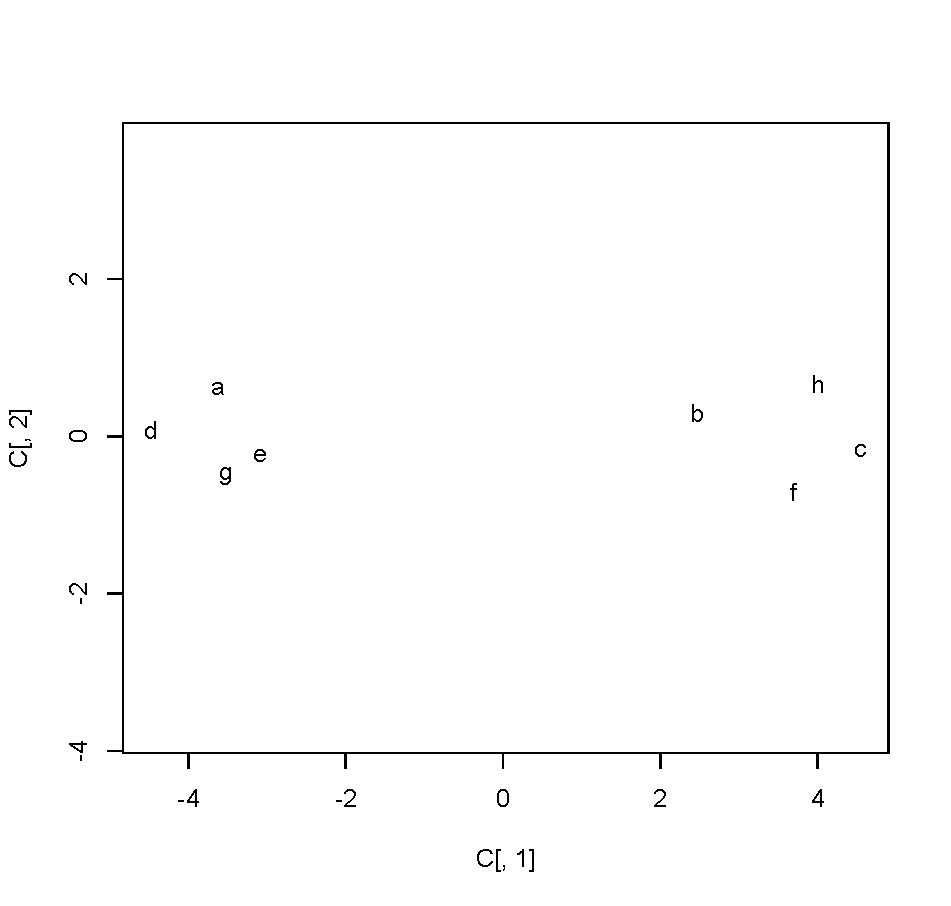
\includegraphics[width=.6\textwidth]{Exo1/ACP.pdf}
\end{center}
\end{figure}
\noindent Dans le plan factoriel, l'ACP transforme donc notre jeu de donnee de $R^2$ suivant l'axe le plus explicatif : le premier. Ceci coincide bien avec les calculs d'inertie expliquee faits a la question 1 : c'est le premier axe qui explique la quasi totalite des donnees.\\

\subsubsection{Calcul de reconstitution} 

\noindent On cherche a calculer l'expression $R = \sum_{\alpha =1}^{k} c_{\alpha} u_{\alpha}^{T}$ selon la valeur de $k$. Nous avons :

- k = 1 : 
\begin{center}
$R = \begin{pmatrix}
3.070960&-1.925643\\
-2.093209&1.312545\\
-3.844996&2.411002\\
3.788736&-2.375725\\
2.620878&-1.643420\\
-3.127220&1.960921\\
2.979766&-1.868461\\
-3.394915&2.128779\\
\end{pmatrix}$
\end{center}

- k = 2 :
\begin{center}
$R = \begin{pmatrix}
2.75&-2.4375 \\
2.25&1.0625 \\
3.75&2.5625 \\
3.75&-2.4375 \\
2.75&-1.4375 \\
-2.75&2.5625 \\
3.25&-1.4375 \\
-3.75&1.5625 \\
\end{pmatrix}$
\end{center}

\noindent On retrouve bien la formule de reconstitution : $Xcentre = CU^T$.


\subsection{MDS}

\subsubsection{ Calcul de la matrice de distance $D^2$}
 
\noindent - Methode A : D2 = dist(Xc, diag=TRUE, upper=TRUE)\\
\noindent - Methode B : D2 = D2proc(X) avec :\\

\noindent D2proc <- function(X)

n <- dim(X)[1];

D2 <- matrix(0,n,n)

for(i in 1: n)

\hspace{1cm}for(j in 1: n)

\hspace{2cm} D2[i,j] <- $(X[i,1] - X[j,1])^2 + (X[i,2] - X[j,2])^2;$

return(D2);\\

\noindent On obtient : 
\begin{center}
$D^2 = \begin{pmatrix}
0.00&37.25&67.25&1.00&1.00&55.25&1.25&58.25\\
37.25&0.00&4.50&48.25&31.25&2.50&36.50&2.50\\
67.25&4.50&0.00&81.25&58.25&1.00&65.00&1.00\\
1.00&48.25&81.25&0.00&2.00&67.25&1.25&72.25\\
1.00&31.25&58.25&2.00&0.00&46.25&0.25&51.25\\
55.25&2.50&1.00&67.25&46.25&0.00&52.00 &2.00\\
1.25&36.50&65.00&1.25&0.25&52.00&0.00&58.00\\
58.25&2.50&1.00&72.25&51.25&2.00&58.00&0.00\\
\end{pmatrix}$
\end{center}

\subsubsection{Calcul de la matrice des produits scalaires}

\noindent On rappelle les notations : $Q_8 = I_8 - \frac{1}{8} U_8$, $X_c = Q_8 X$, nous avons les relations suivantes :\\

-  Methode A : Calcul direct a partir de X centree : $W = X_c  X_c^T$, (par definition)

- Methode B : Caclul de W a partir de $D^2$ : $W = -\frac{1}{2} Q_n  D^2  Q_n^T$\\

Par ces 2 methodes, on obtient la matrice des produits scalaires W : 
\begin{center}
$\begin{pmatrix}
13.503906&-8.777344&-16.55859&16.25391&11.066406&-13.808594&12.441406&-14.12109\\
-8.777344&6.191406&11.16016&-11.02734&-7.714844&8.910156&-8.839844&10.09766\\
-16.558594&11.160156&20.62891&-20.30859&-13.996094&16.878906&-15.871094&18.06641\\
16.253906&-11.027344&-20.30859&20.00391&13.816406&-16.558594&15.691406&-17.87109\\
11.066406&-7.714844&-13.99609&13.81641&9.628906&-11.246094&11.003906&-12.55859\\
-13.808594&8.910156&16.87891&-16.55859&-11.246094&14.128906&-12.621094&14.31641\\
12.441406&-8.839844&-15.87109&15.69141&11.003906&-12.621094&12.628906&-14.43359\\
-14.121094&10.097656&18.06641&-17.87109&-12.558594&14.316406&-14.433594&16.50391\\
\end{pmatrix}$
\end{center}

\subsubsection{W, matrice semi-definie positive}

\noindent Soit $\lambda_i$ les valeurs propres d'une matrice A. Alors nous savons que $(0 \le \lambda_i)$ est une condition necessaire pour que A soit semi definie positive.\\

\noindent Or si nous calculons les valeurs propres de W, nous avons :
\begin{center}
$\begin{pmatrix}
1.114606e+02\\
1.758189e+00\\
1.253786e-15\\
3.542804e-16\\
3.517163e-16\\
2.647375e-16\\
-4.348568e-15\\
-6.257752e-15\\
\end{pmatrix}$
\end{center}
\noindent En ne tenant pas compte des erreurs d'arrondis pour les 2 dernieres valeurs propres de W ($\approx 0)$, nous observons que ces dernieres sont toutes positives ou nulles. La matrice W est donc semi definie positive.

\subsubsection{Matrice des vecteurs propres normes V et matrice des valeurs propres L}

\noindent Nous realisons l'analyse spectrale de la matrice des produits scalaires normees $W_8 = \frac{1}{8} W$\\
\noindent Soit Va = valeur propres($W_8$) et Ve = vecteurs propres($W_8$), nous avons :

$L = \left| Va \right| $, matrice 1 x 8.

$V = \sqrt{8}$ Ve, matrice 8 x 8.\\

\noindent On obtient les matrices de l'AFTD suivantes : 
\begin{center}
$L^T = \begin{pmatrix}
1.393257e+01\\
2.197736e-01\\
1.567232e-16\\
4.428506e-17\\
4.396454e-17\\
3.309219e-17\\
5.435710e-16\\
7.822190e-16
\end{pmatrix}$
\end{center}

\hspace{-2.8cm} $V = \begin{pmatrix}
0.9710996&1.2887422&0.0000000&0.00000000&0.00000000&0.00000000&2.32295266&0.00000000\\
-0.6619152&0.6295590&-0.3296600&-0.15663742&-0.42496324&-0.08830037&-0.07256009&-2.61508264\\
-1.2158658&-0.3814373&-0.5057538&-0.81531004&1.10304156&-1.91912099&0.71990321&0.19409265\\
1.1980752&0.1555369&-1.2288345&-1.37201816&1.48486894&0.72183755&-0.58713952&-0.27809748\\
0.8287747&-0.5184606&-2.0705045&0.92993122&-1.04673363&-0.88781302&-0.05883065&0.07242854\\
-0.9888902&-1.5146425&-0.7565655&0.02216901&0.04585093&1.60237091&1.25370385&-0.11663199\\
0.9422625&-1.0850632&0.7243776&1.50962793&1.45096368&-0.39354572&0.20806967&-0.90973232\\
-1.0735409&1.4257655&-0.8610459&1.51131083&1.09307849&0.52673093&-0.34220630&0.44706917\\
\end{pmatrix}$\\
\\

\subsubsection{Representation de l AFTD}

\noindent Nous representons d'une part le nuage associe au tableau initial X et d'autre part le nuage associe a la representation fournie par l'AFTD

\hspace{-1.8cm} 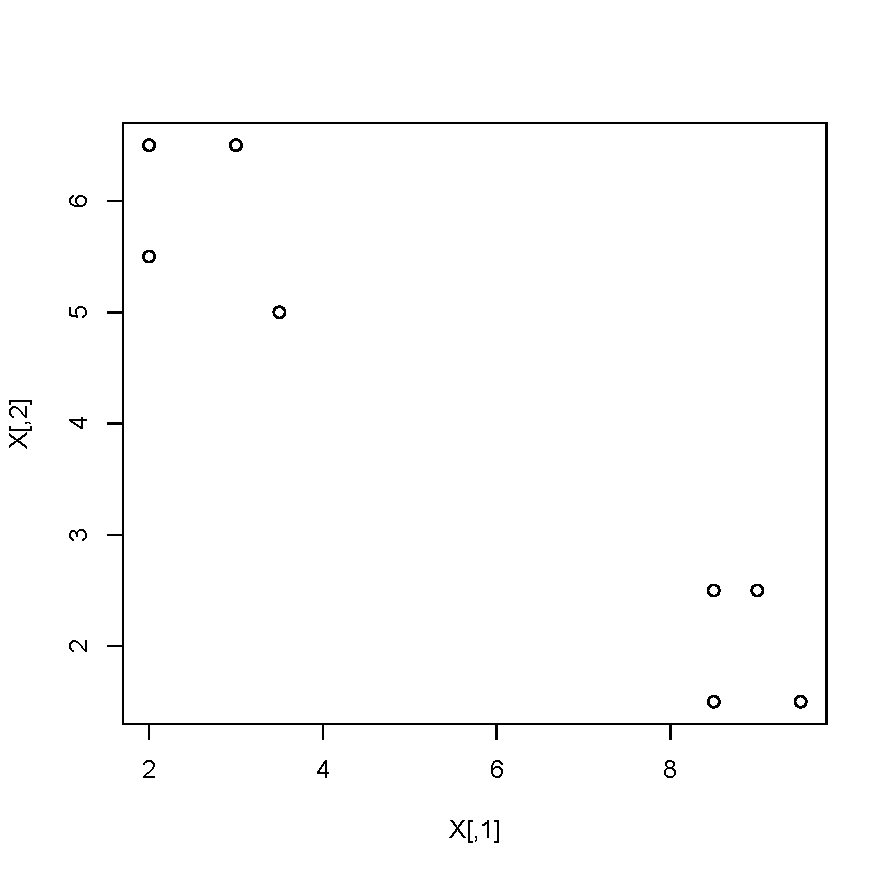
\includegraphics[width=.6\textwidth]{Exo1/plot_X_MDS.pdf}
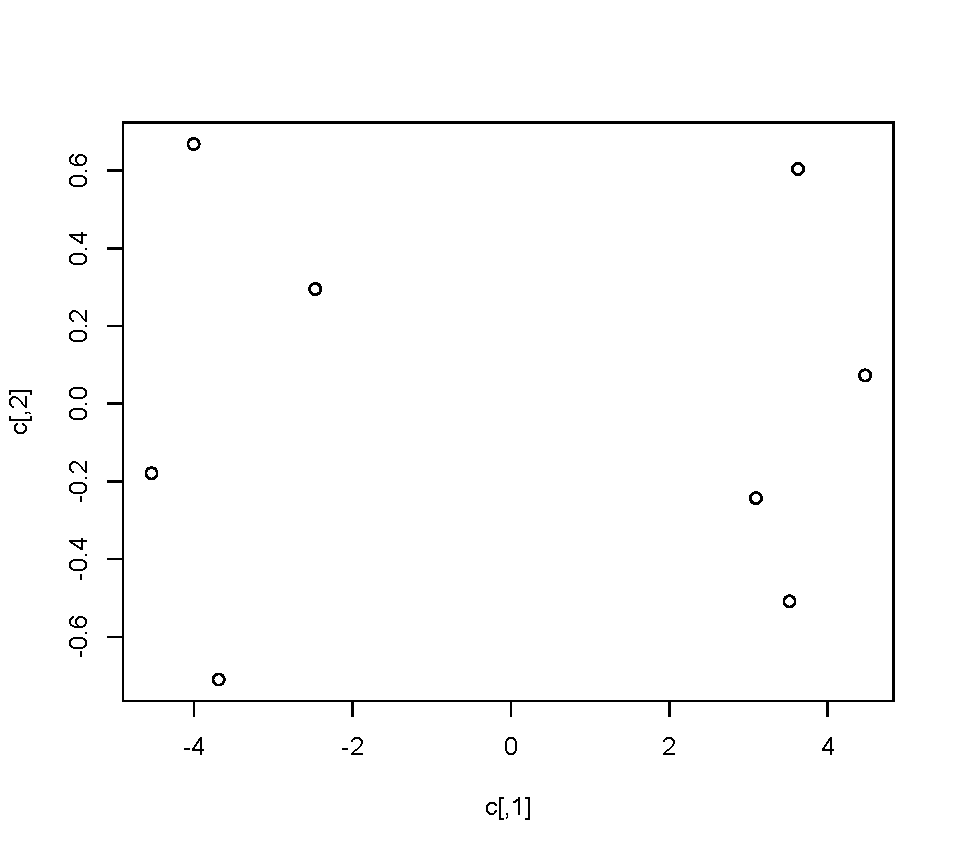
\includegraphics[width=.6\textwidth]{Exo1/plot_MDS.pdf}\\

\noindent La premiere representation nous donne clairement 2 groupes d'individus bien separes. La representation par l'AFTD nous donne plus de precision quant a la separation de ces donnees. En effet, le deuxieme graphique nous informe que les donnees different principalement selon le premier axe alors qu'elles sont a peu pres toutes confondues sur le deuxieme axe. Ceci confirme bien les resultats de l'ACP sur l'explication des donnes par le premier axe par rapport au deuxieme.

\subsubsection{Fonction donnant la representation par l'AFTD d'une matrice de distance D passee en parametre}
\hspace{2cm}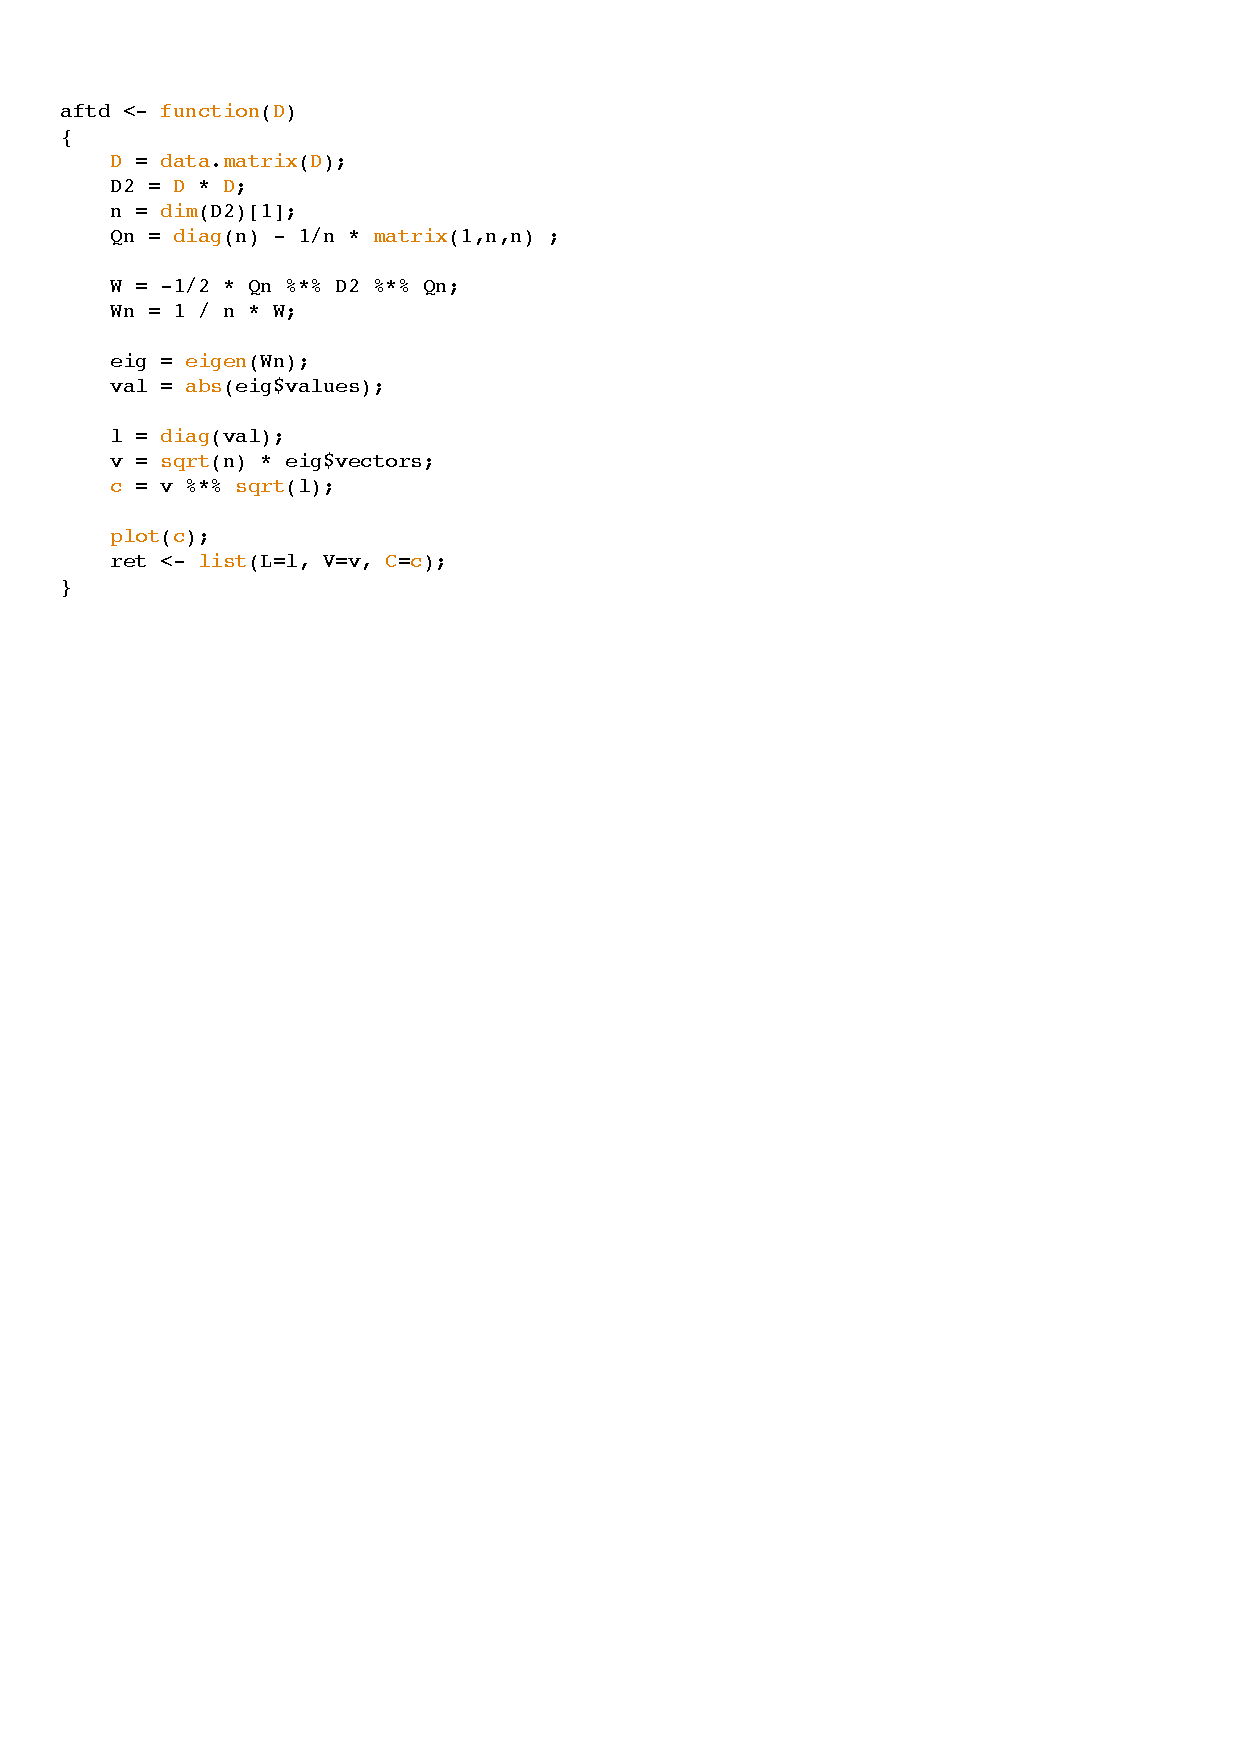
\includegraphics[width=.6\textwidth]{Exo1/aftd.pdf}\\
\\

\section{Les donnees de mutations}

\subsection{AFTD}

\noindent Voici les resultats utilises avec les 2 methodes (a gauche notre fonction "maison", a droite la fonciton R $cmdscale$)

\hspace{-1.8cm} 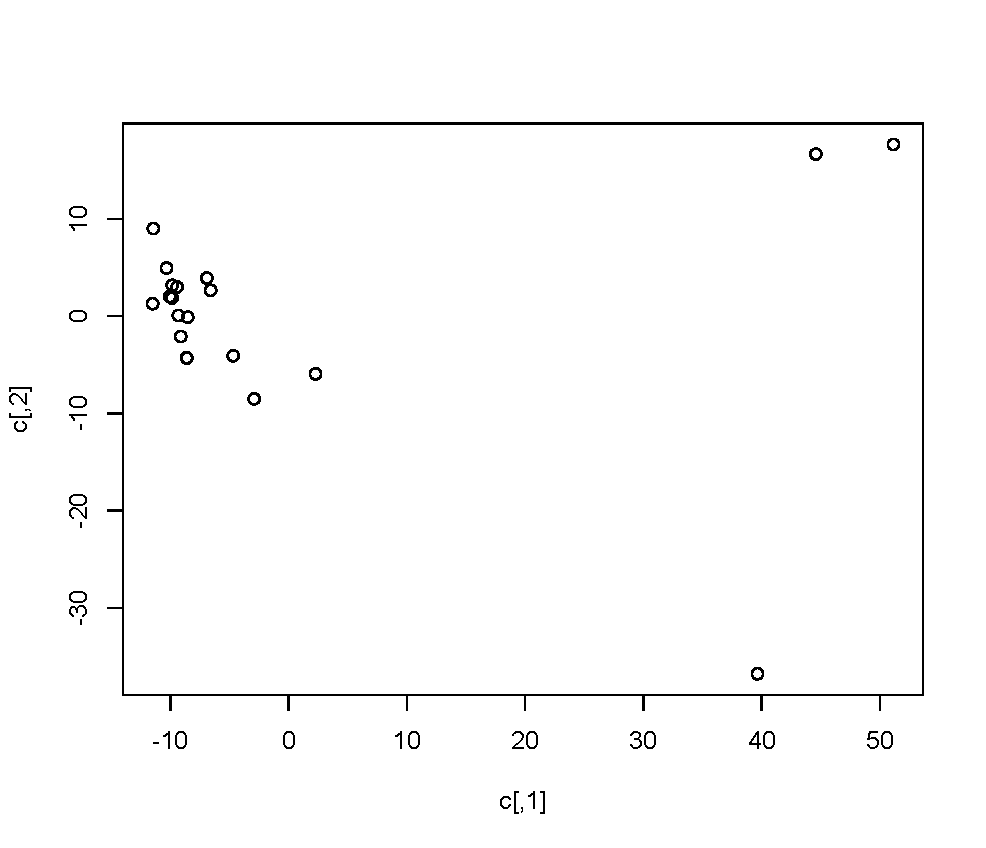
\includegraphics[width=.6\textwidth]{Exo2/aftd1.pdf}
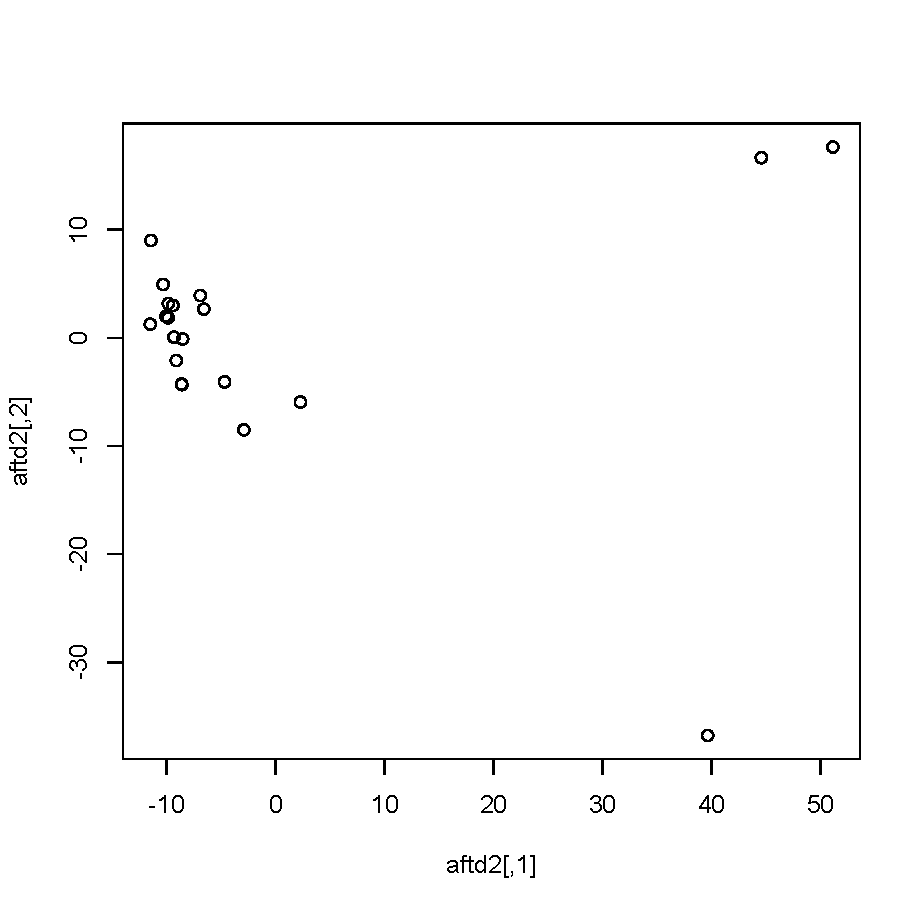
\includegraphics[width=.6\textwidth]{Exo2/cmdscale.pdf}\\

\noindent Les 2 representations obtenues sont identiques : les 2 fonctions utilisent la meme methode.\\

\subsection{Projections de Sammon et de Kruskal}

\noindent Commencons par comparer l'AFTD et la projection de Sammon : Si on note les distances entre $i$ et $j$ dans la matrice de depart par $d_{ij}$ et la distance entre leur projections par $\delta_{i,j}$. La projection de Sammon a pour but de minimiser la fonction d'ecart (stress) suivante :

\begin{equation}
Stress = \frac{1}{\sum\limits_{i<j} d_{ij}} \sum\limits_{i<j} \frac{ ( d_{ij} - \delta_{ij} )^2 }{d_{ij}}
\end{equation}

\hspace{-.8cm} \includegraphics[width=0.95\textwidth]{Exo2/sammon1.pdf}\\

\noindent La projection de Sammon (ci-dessus) ameliore la representation. Les distances semblent plus fidelement representees. Pour illustrer ce propos, le fonction stress ci-dessus renvoyait 0.2 initialement (donc pour l'AFTD) et 0.02 a la fin. Ceci illustre le fait que la representation s'est amelioree.

\begin{center}
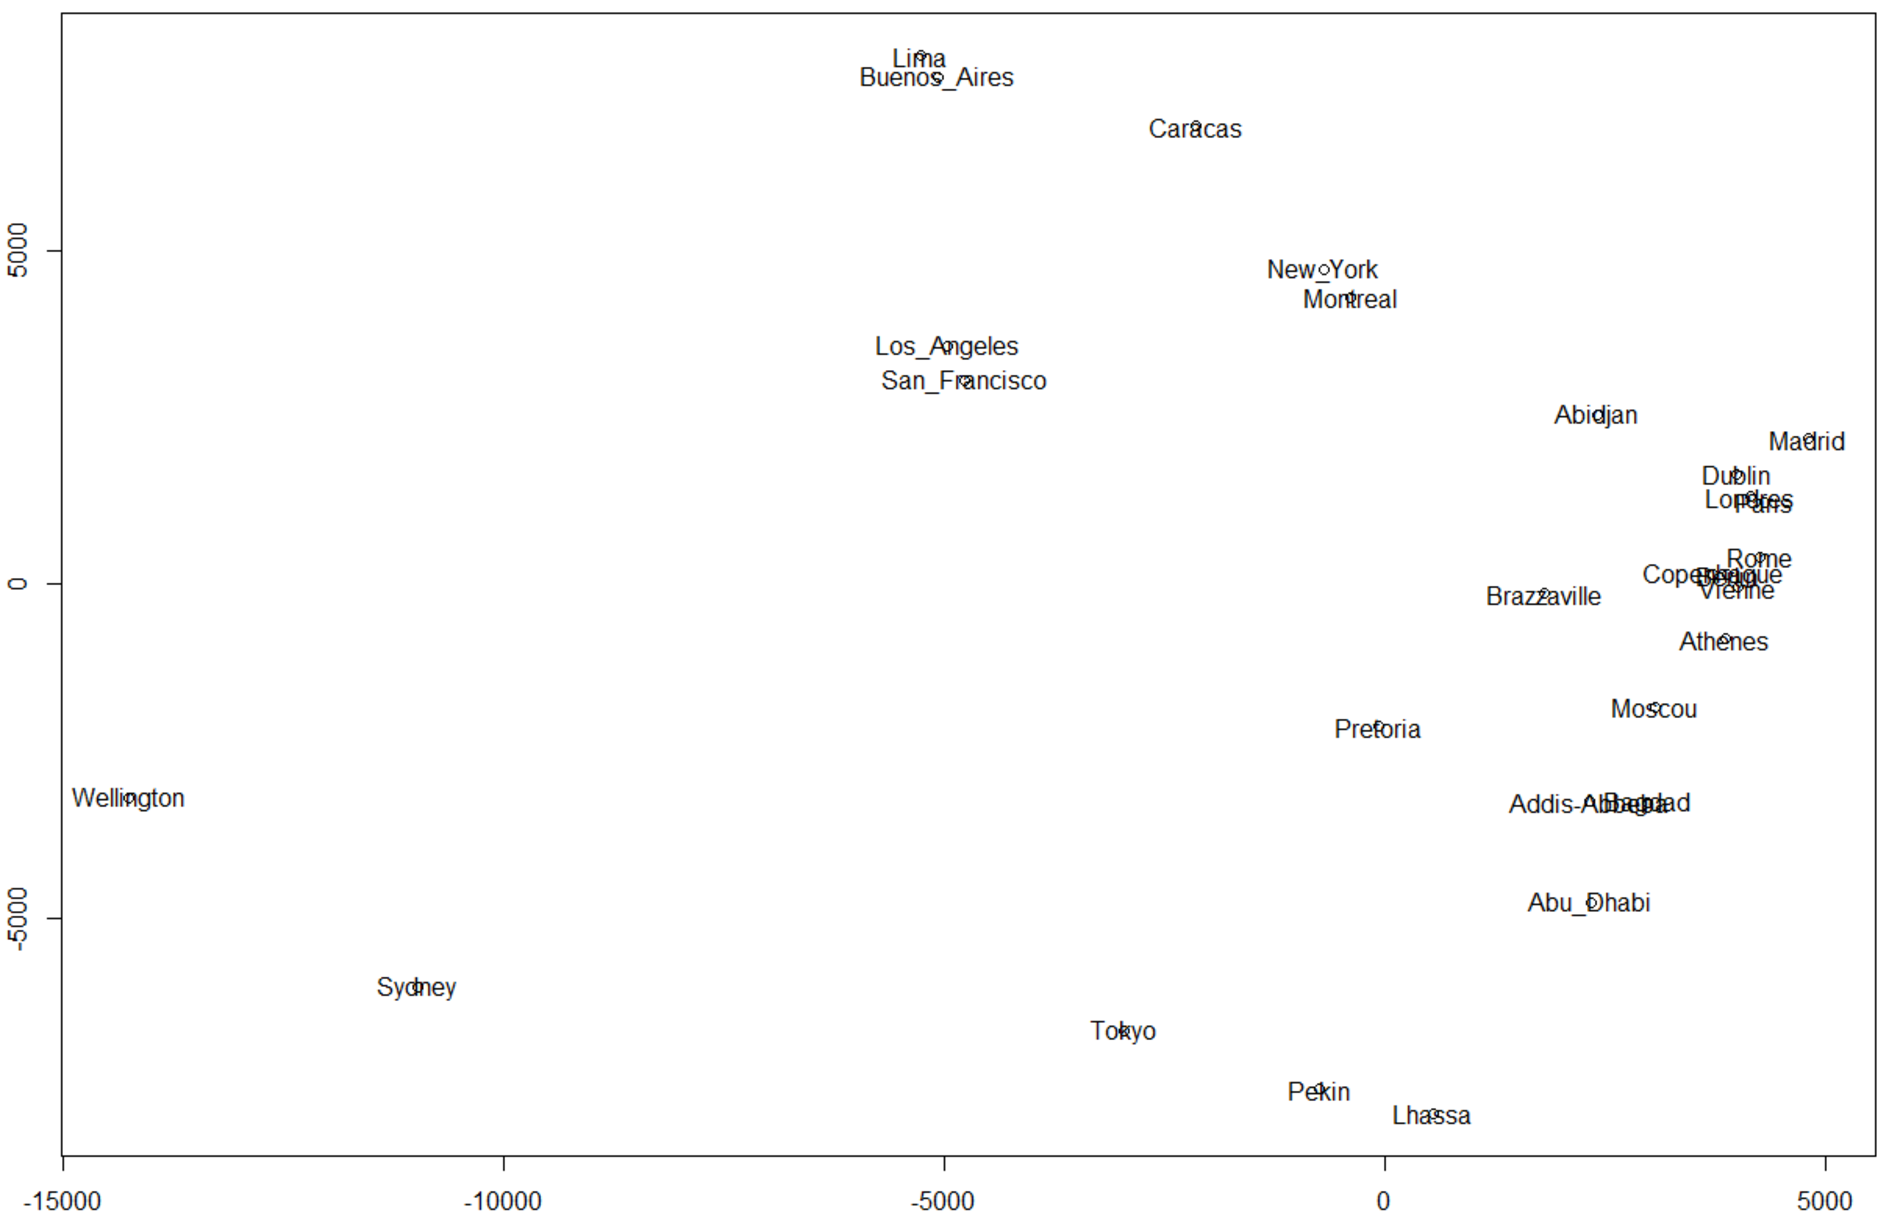
\includegraphics[width=0.6\textwidth]{Exo2/Kruskal.pdf}\\
\end{center}

\noindent L'idee sous-jacente a la projection de Kruskal (ci-dessus) est qu'en negligeant le lien entre la dissimilarite et la distance obtenue, le resultat sera plus fidele.
Cette representation nous permet de regrouper les especes en 3 familles mais rien de plus. Par rapport a l'AFTD, nous perdons de l'information puisqu'on ne peut plus faire de difference a l'interieur des groupes.\\
\\

\subsection{Diagramme de Shepard}

\hspace{-1.8cm} 
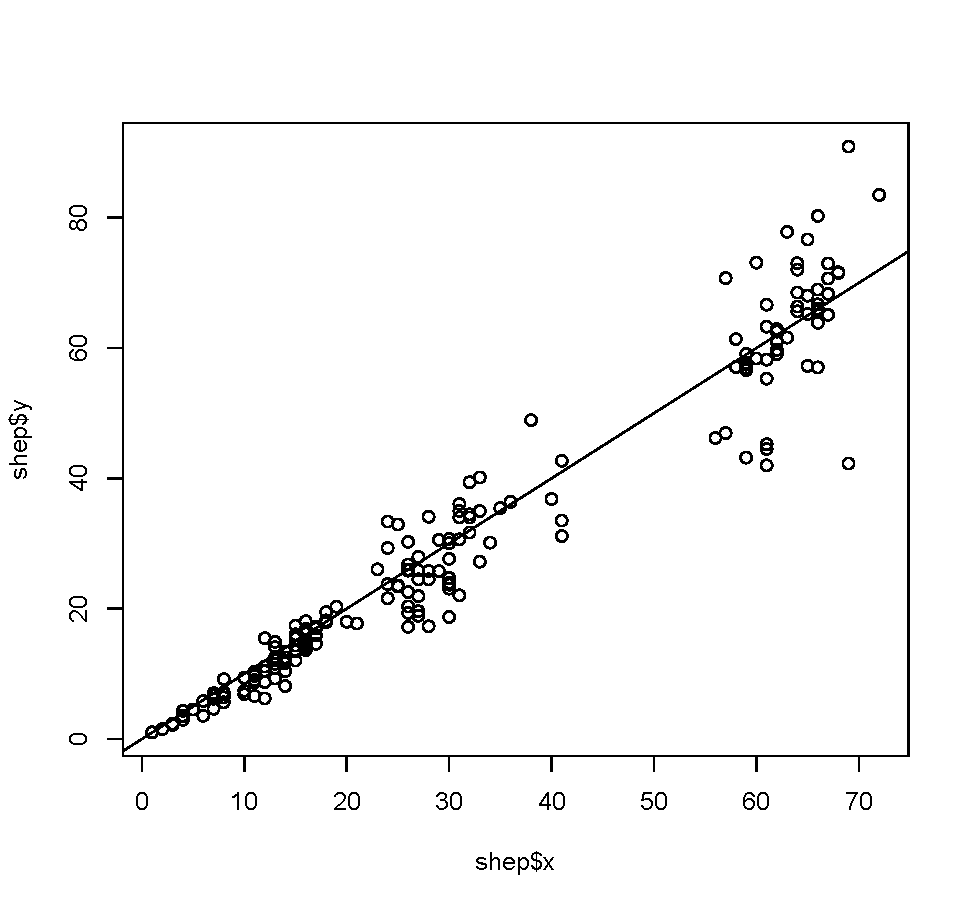
\includegraphics[width=.6\textwidth]{Exo2/shep-sam.pdf}
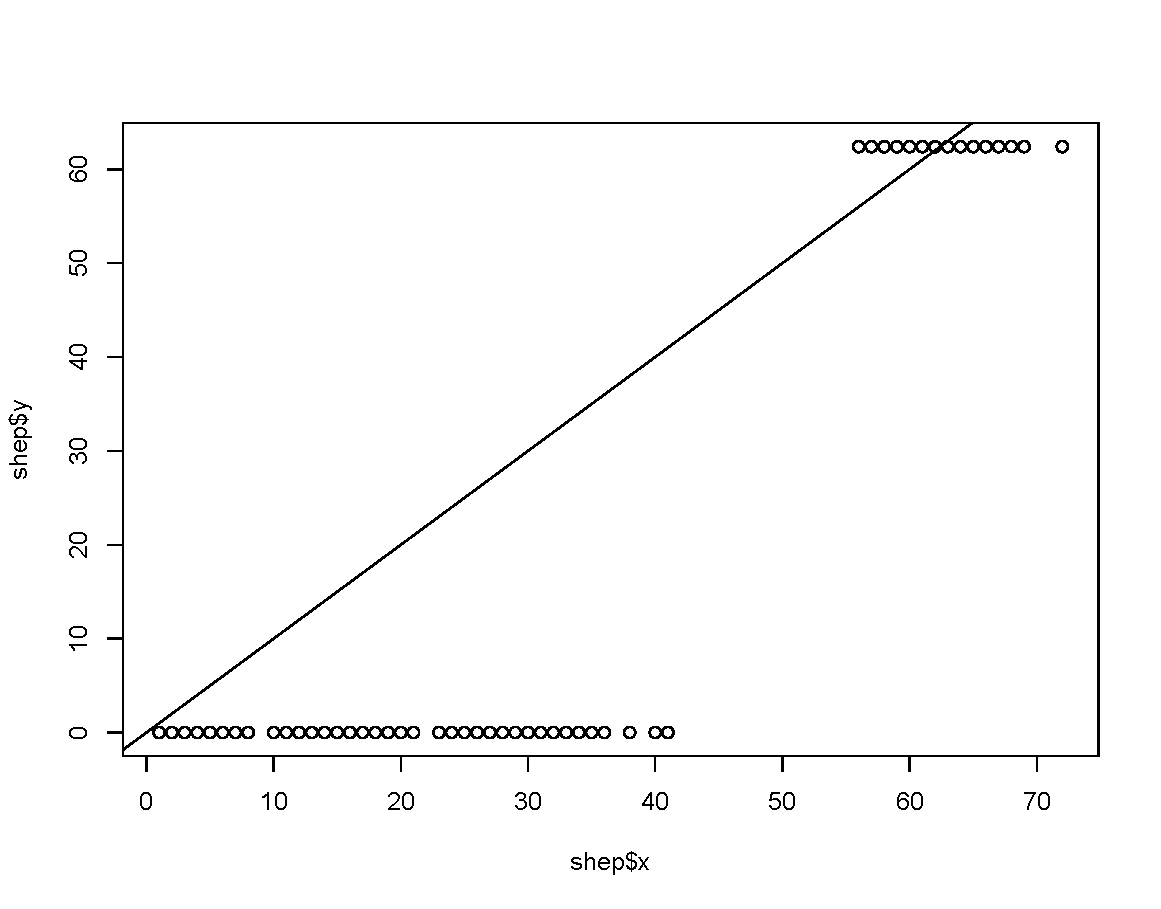
\includegraphics[width=.6\textwidth]{Exo2/shep.pdf}\\

\noindent On remarque que sur le diagramme de Shepard de la projection de Sammon (a gauche), les points sont assez prets de la bissectrice, ce qui indique que les distances initiales ont plutot bien ete retranscrites dans cette projection. Sur les autres diagrammes de Shepard (par exemple a droite), les points sont beaucoup plus loin de cette bissectrice.\\
\\

\section{Les donnees de distances entre aeroport}

\subsection{AFTD}

\noindent La representation des donnees par l'AFTD nous donne une sorte de carte du monde. Cette representation n'est neanmoins pas tout a fait exacte. Par exemple, Brazzaville (Congo) est a la meme distance de Londres que de Buenos Aires. Sur la representation obtenue par AFTD, Londres est entre 4 et 5 fois plus proche de Buenos Aires que Brazzaville. \\

\noindent Ceci peut provenir du fait que les donnes traitent des distances de vol, c'est a dire des distances non planes.\\

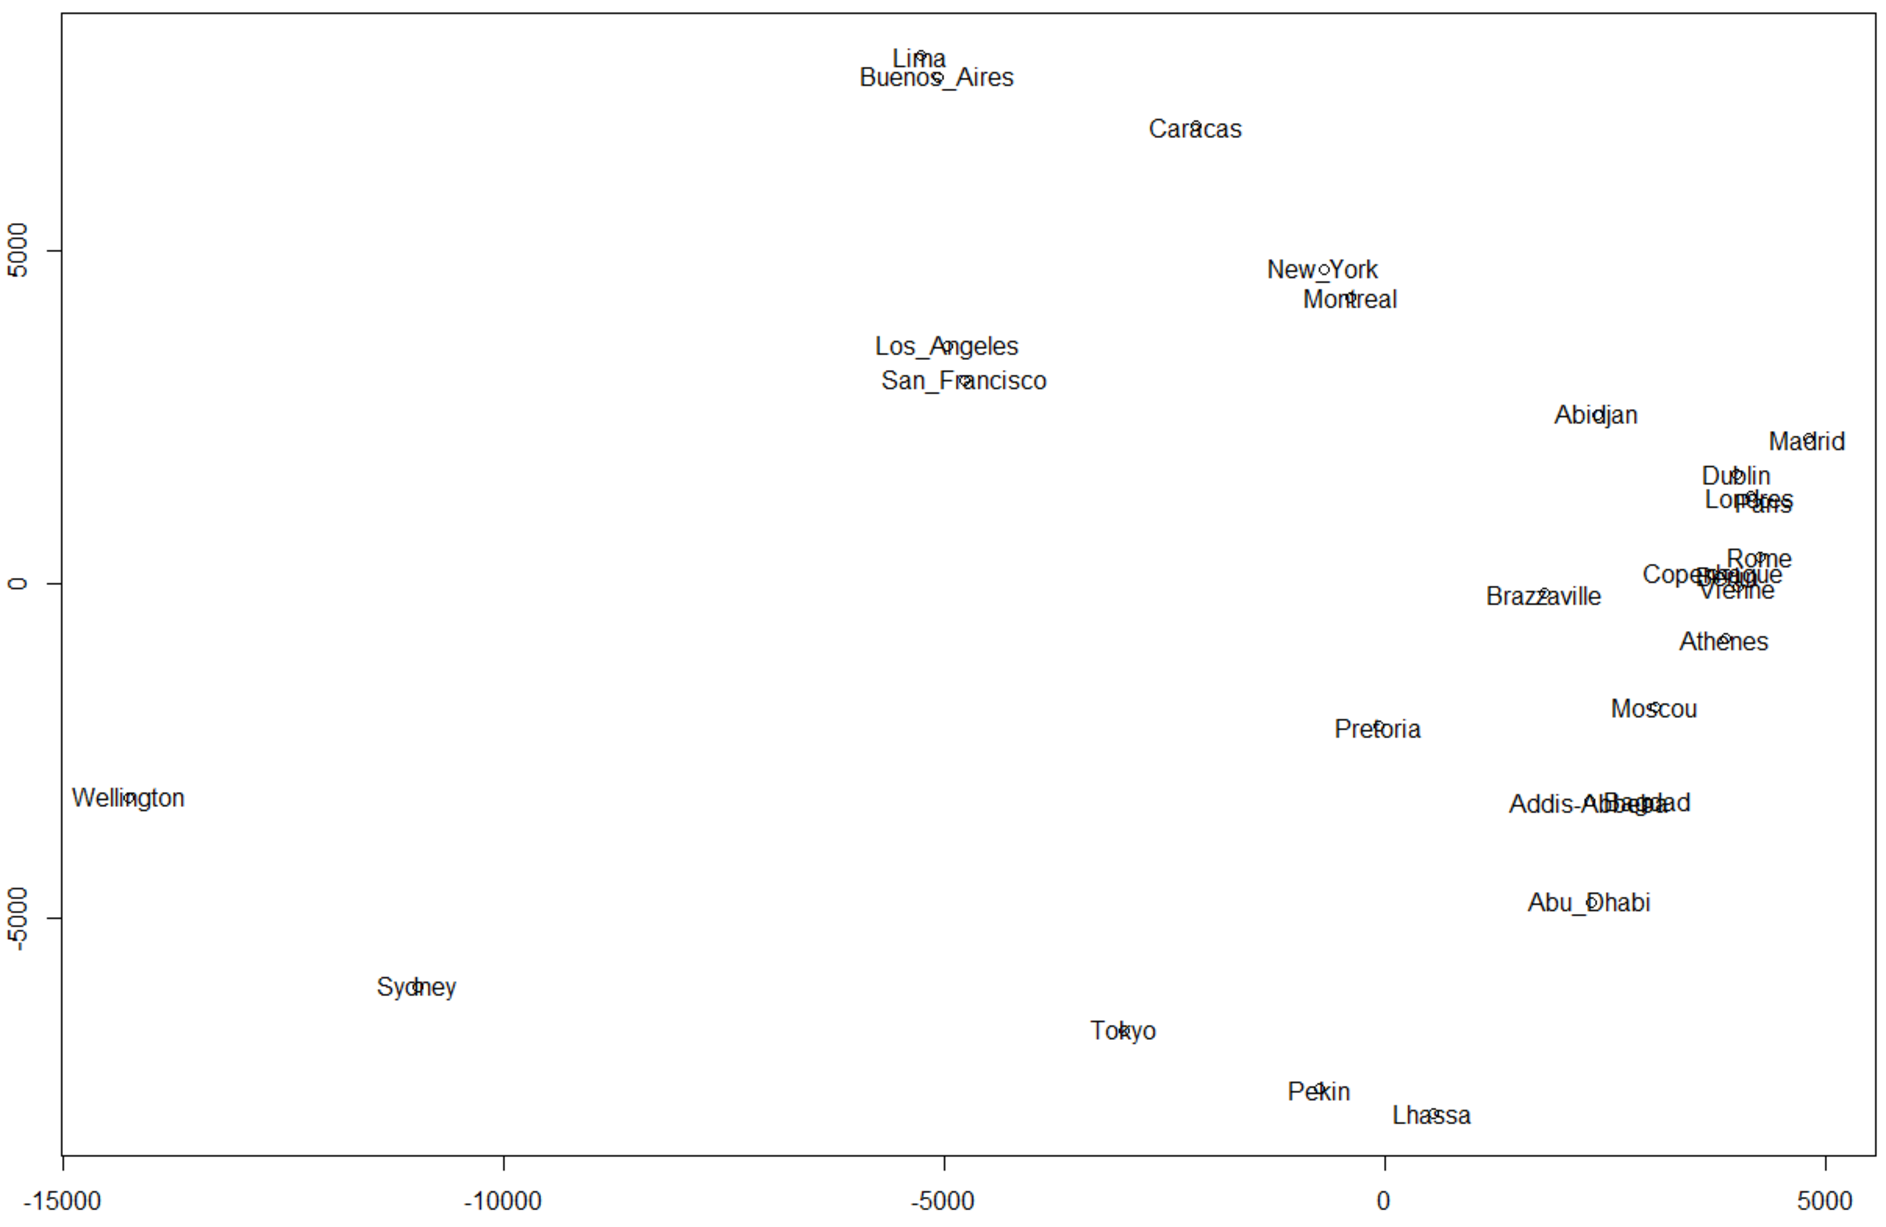
\includegraphics[width=.9\textwidth]{Exo3/aftd.pdf}\\
\\

\subsection{Projections de Sammon et de Kruskal}

\noindent La representation issue de la projection de Sammon (a gauche) semble plus fidele a la realite (et aux donnees fournies). Par exemple, la distance entre Londre et Brazzaville a augmentee alors que celle entre Brazzaville et Buenos Aires est restee identique. Le stress initial (de l'AFTD) etait de 0.6 et le stress final de 0.4 : Il y a donc eu peu d'amelioration. \\
Ce stress reste important du fait des distances non planes (plutot spherique).\\

\noindent Entre la representation issue de la projection de Kruskal (a droite) et la representation issue de l'AFTD, il ne semble pas y avoir de difference. Les 2 diagrammes de Shepard pour chacune de ces representations sont quasi identiques.
A la vue des diagrammes de Shepard, il est difficile de dire quelle representation des 3 est la meilleure.\\

\hspace{-2.3cm} 
\includegraphics[width=.6\textwidth]{Exo3/sammon.pdf}
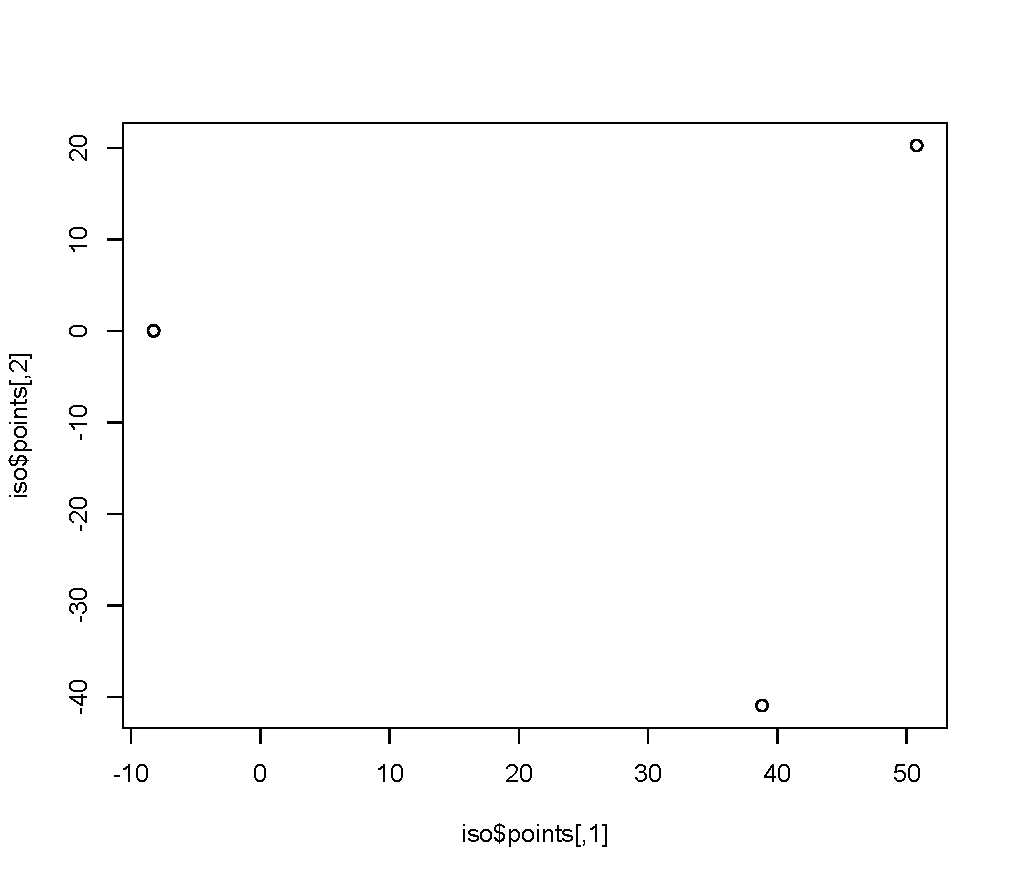
\includegraphics[width=.6\textwidth]{Exo3/kruskal.pdf}\\

\subsection{Aeroports europeens}

\noindent En effectuant l'AFTD des donnees restreintes aux aeroports Europeens, on observe des resultats tres proches de la realite. Le diagramme de Shepard "Europe" (a gauche) nous donne une representation quasi "parfaite" :  tous les points sont alignes sur la bissectrice. Nous pouvons comparer ce digramme avec celui du monde, a droite :

\hspace{-2.3cm} 
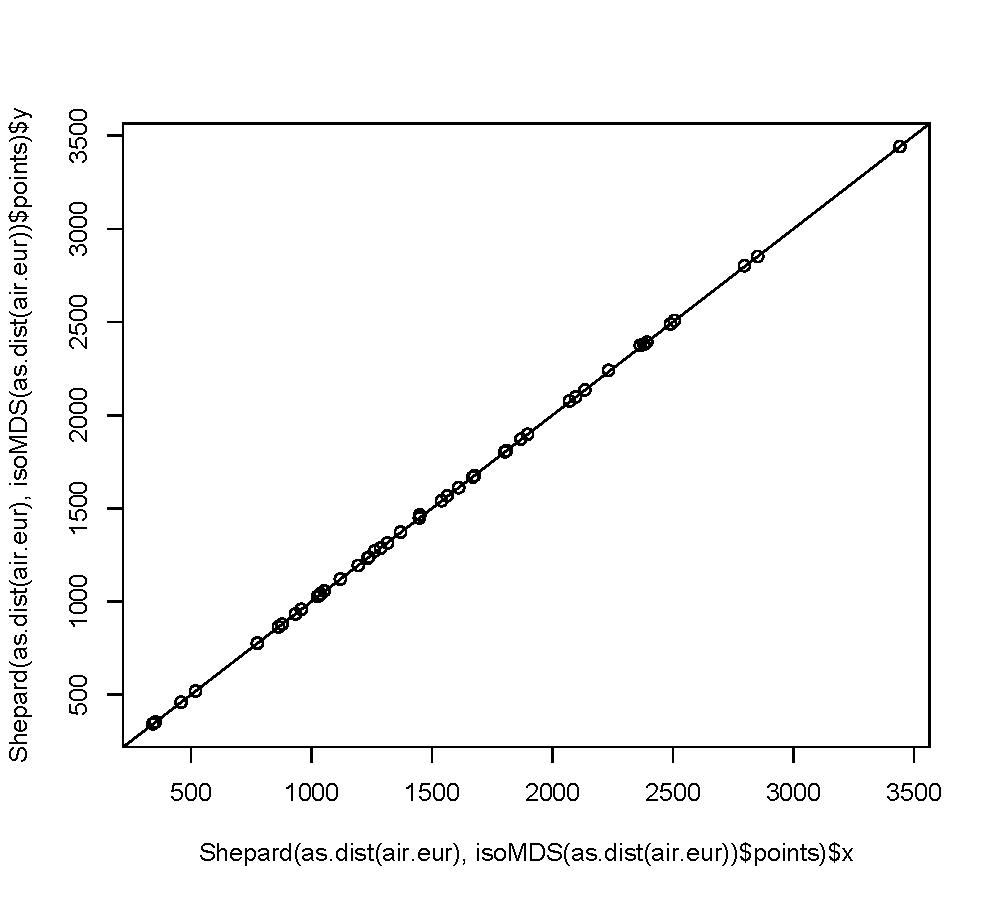
\includegraphics[width=.6\textwidth]{Exo3/shep-eur.pdf}
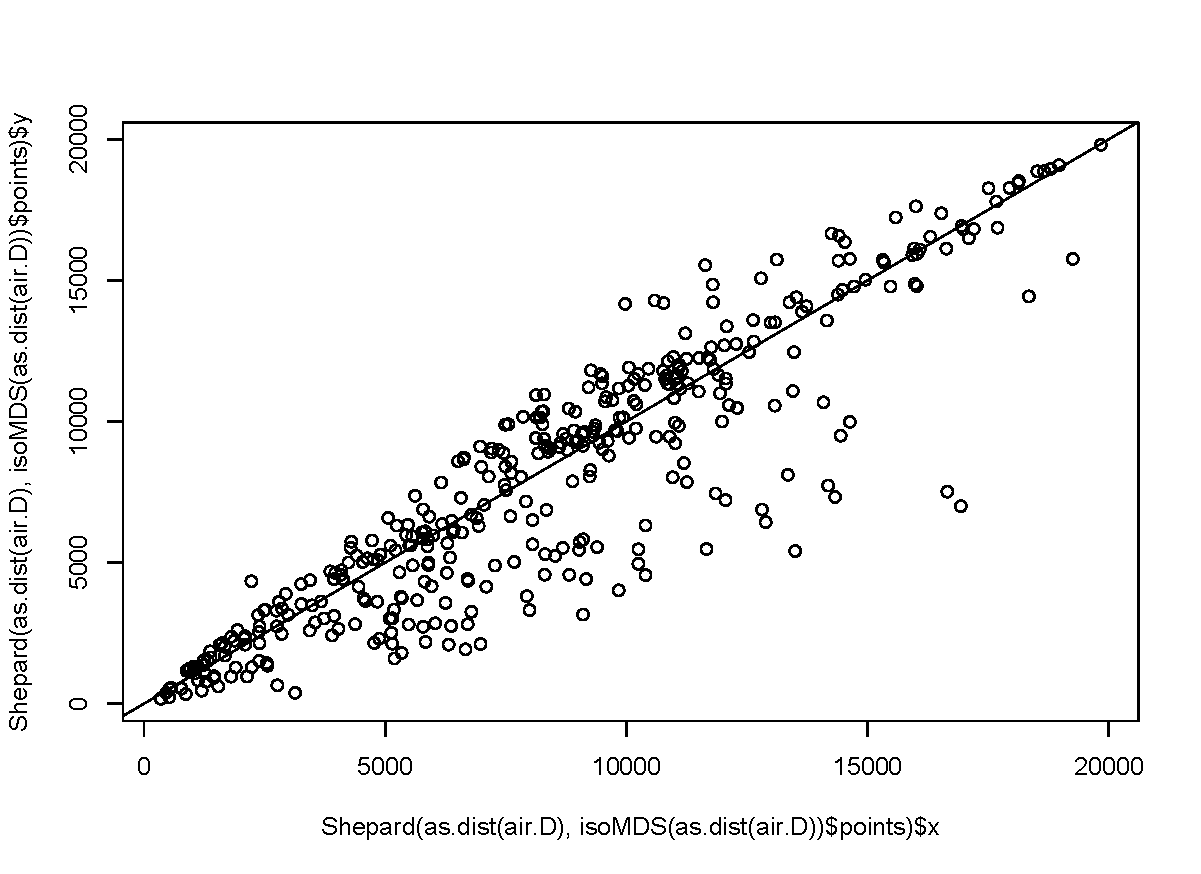
\includegraphics[width=.6\textwidth]{Exo3/shep-monde.pdf}\\

\noindent Lorsque l'on se restreint a l'Europe, les distance traitees sont moindres. Ainsi les distances de vol peuvent etre assimilees a celles d'un plan. \\
Nous obtenons donc de bons resultats car toutes les representations effectuees sont soumises a l'hypothese de distances euclidiennes. Ces hyptoheses  etait moins verifiees pour la matrice de distance associee au monde entier.\\
\\

\section{Conclusion}
\noindent Quelque soit les donnees du probleme : $p$ mesures de $n$ variables pour l'ACP ou tableau de distance pour l'AFTD, les techniques de positionnement mutlidimensionnel permettent, de maniere efficace, la representation en dimension reduite d'un jeu de donnees.\\

\noindent A travers l'exercice theorique, nous avons pu apprecier la puissance de l'ACP pour expliquer a travers un seul axe l'ensemble des donnees. D'autre part, apres avoir realise une fonction smilaire a $cmdscale$ afin de mieux en comprendre le mecanisme, nous avons pu appliquer l'AFTD a 2 jeux de donnees bien differents. \\

\noindent A chaque fois les differentes projections nous ont permis de visualiser ces donnees dans $R^2$ afin de mieux "toucher du doigt" ces donnees et ainsi comparer ces representations avec celle de l'AFTD.\\
Enfin c'est le diagramme de Shepard qui nous a, a chaque fois, permis de trancher entre ces differentes representations, il en demeure donc tres utile.

\end{document}